\documentclass[11pt,a4paper]{report}
\usepackage[textwidth=37em,vmargin=30mm]{geometry}
\usepackage{calc,xunicode,amsmath,amssymb,paralist,enumitem,tabu,booktabs,datetime2,xeCJK,xeCJKfntef,listings}
\usepackage{tocloft,fancyhdr,tcolorbox,xcolor,graphicx,eso-pic,xltxtra,xelatexemoji}

\newcommand{\envyear}[0]{2025}
\newcommand{\envdatestr}[0]{2025-04-13}
\newcommand{\envfinaldir}[0]{webdb/2025/20250413/final}

\usepackage[hidelinks]{hyperref}
\hypersetup{
    colorlinks=false,
    pdfpagemode=FullScreen,
    pdftitle={Web Digest - \envdatestr}
}

\setlength{\cftbeforechapskip}{10pt}
\renewcommand{\cftchapfont}{\rmfamily\bfseries\large\raggedright}
\setlength{\cftbeforesecskip}{2pt}
\renewcommand{\cftsecfont}{\sffamily\small\raggedright}

\setdefaultleftmargin{2em}{2em}{1em}{1em}{1em}{1em}

\usepackage{xeCJK,xeCJKfntef}
\xeCJKsetup{PunctStyle=plain,RubberPunctSkip=false,CJKglue=\strut\hskip 0pt plus 0.1em minus 0.05em,CJKecglue=\strut\hskip 0.22em plus 0.2em}
\XeTeXlinebreaklocale "zh"
\XeTeXlinebreakskip = 0pt


\setmainfont{Brygada 1918}
\setromanfont{Brygada 1918}
\setsansfont{IBM Plex Sans}
\setmonofont{JetBrains Mono NL}
\setCJKmainfont{Noto Serif CJK SC}
\setCJKromanfont{Noto Serif CJK SC}
\setCJKsansfont{Noto Sans CJK SC}
\setCJKmonofont{Noto Sans CJK SC}

\setlength{\parindent}{0pt}
\setlength{\parskip}{8pt}
\linespread{1.15}

\lstset{
	basicstyle=\ttfamily\footnotesize,
	numbersep=5pt,
	backgroundcolor=\color{black!5},
	showspaces=false,
	showstringspaces=false,
	showtabs=false,
	tabsize=2,
	captionpos=b,
	breaklines=true,
	breakatwhitespace=true,
	breakautoindent=true,
	linewidth=\textwidth
}






\newcommand{\coverpic}[2]{
    % argv: itemurl, authorname
    Cover photo by #2~~(\href{#1}{#1})
}
\newcommand{\makeheader}[0]{
    \begin{titlepage}
        % \newgeometry{hmargin=15mm,tmargin=21mm,bmargin=12mm}
        \begin{center}
            
            \rmfamily\scshape
            \fontspec{BaskervilleF}
            \fontspec{Old Standard}
            \fontsize{59pt}{70pt}\selectfont
            WEB\hfill DIGEST
            
            \vfill
            % \vskip 30pt
            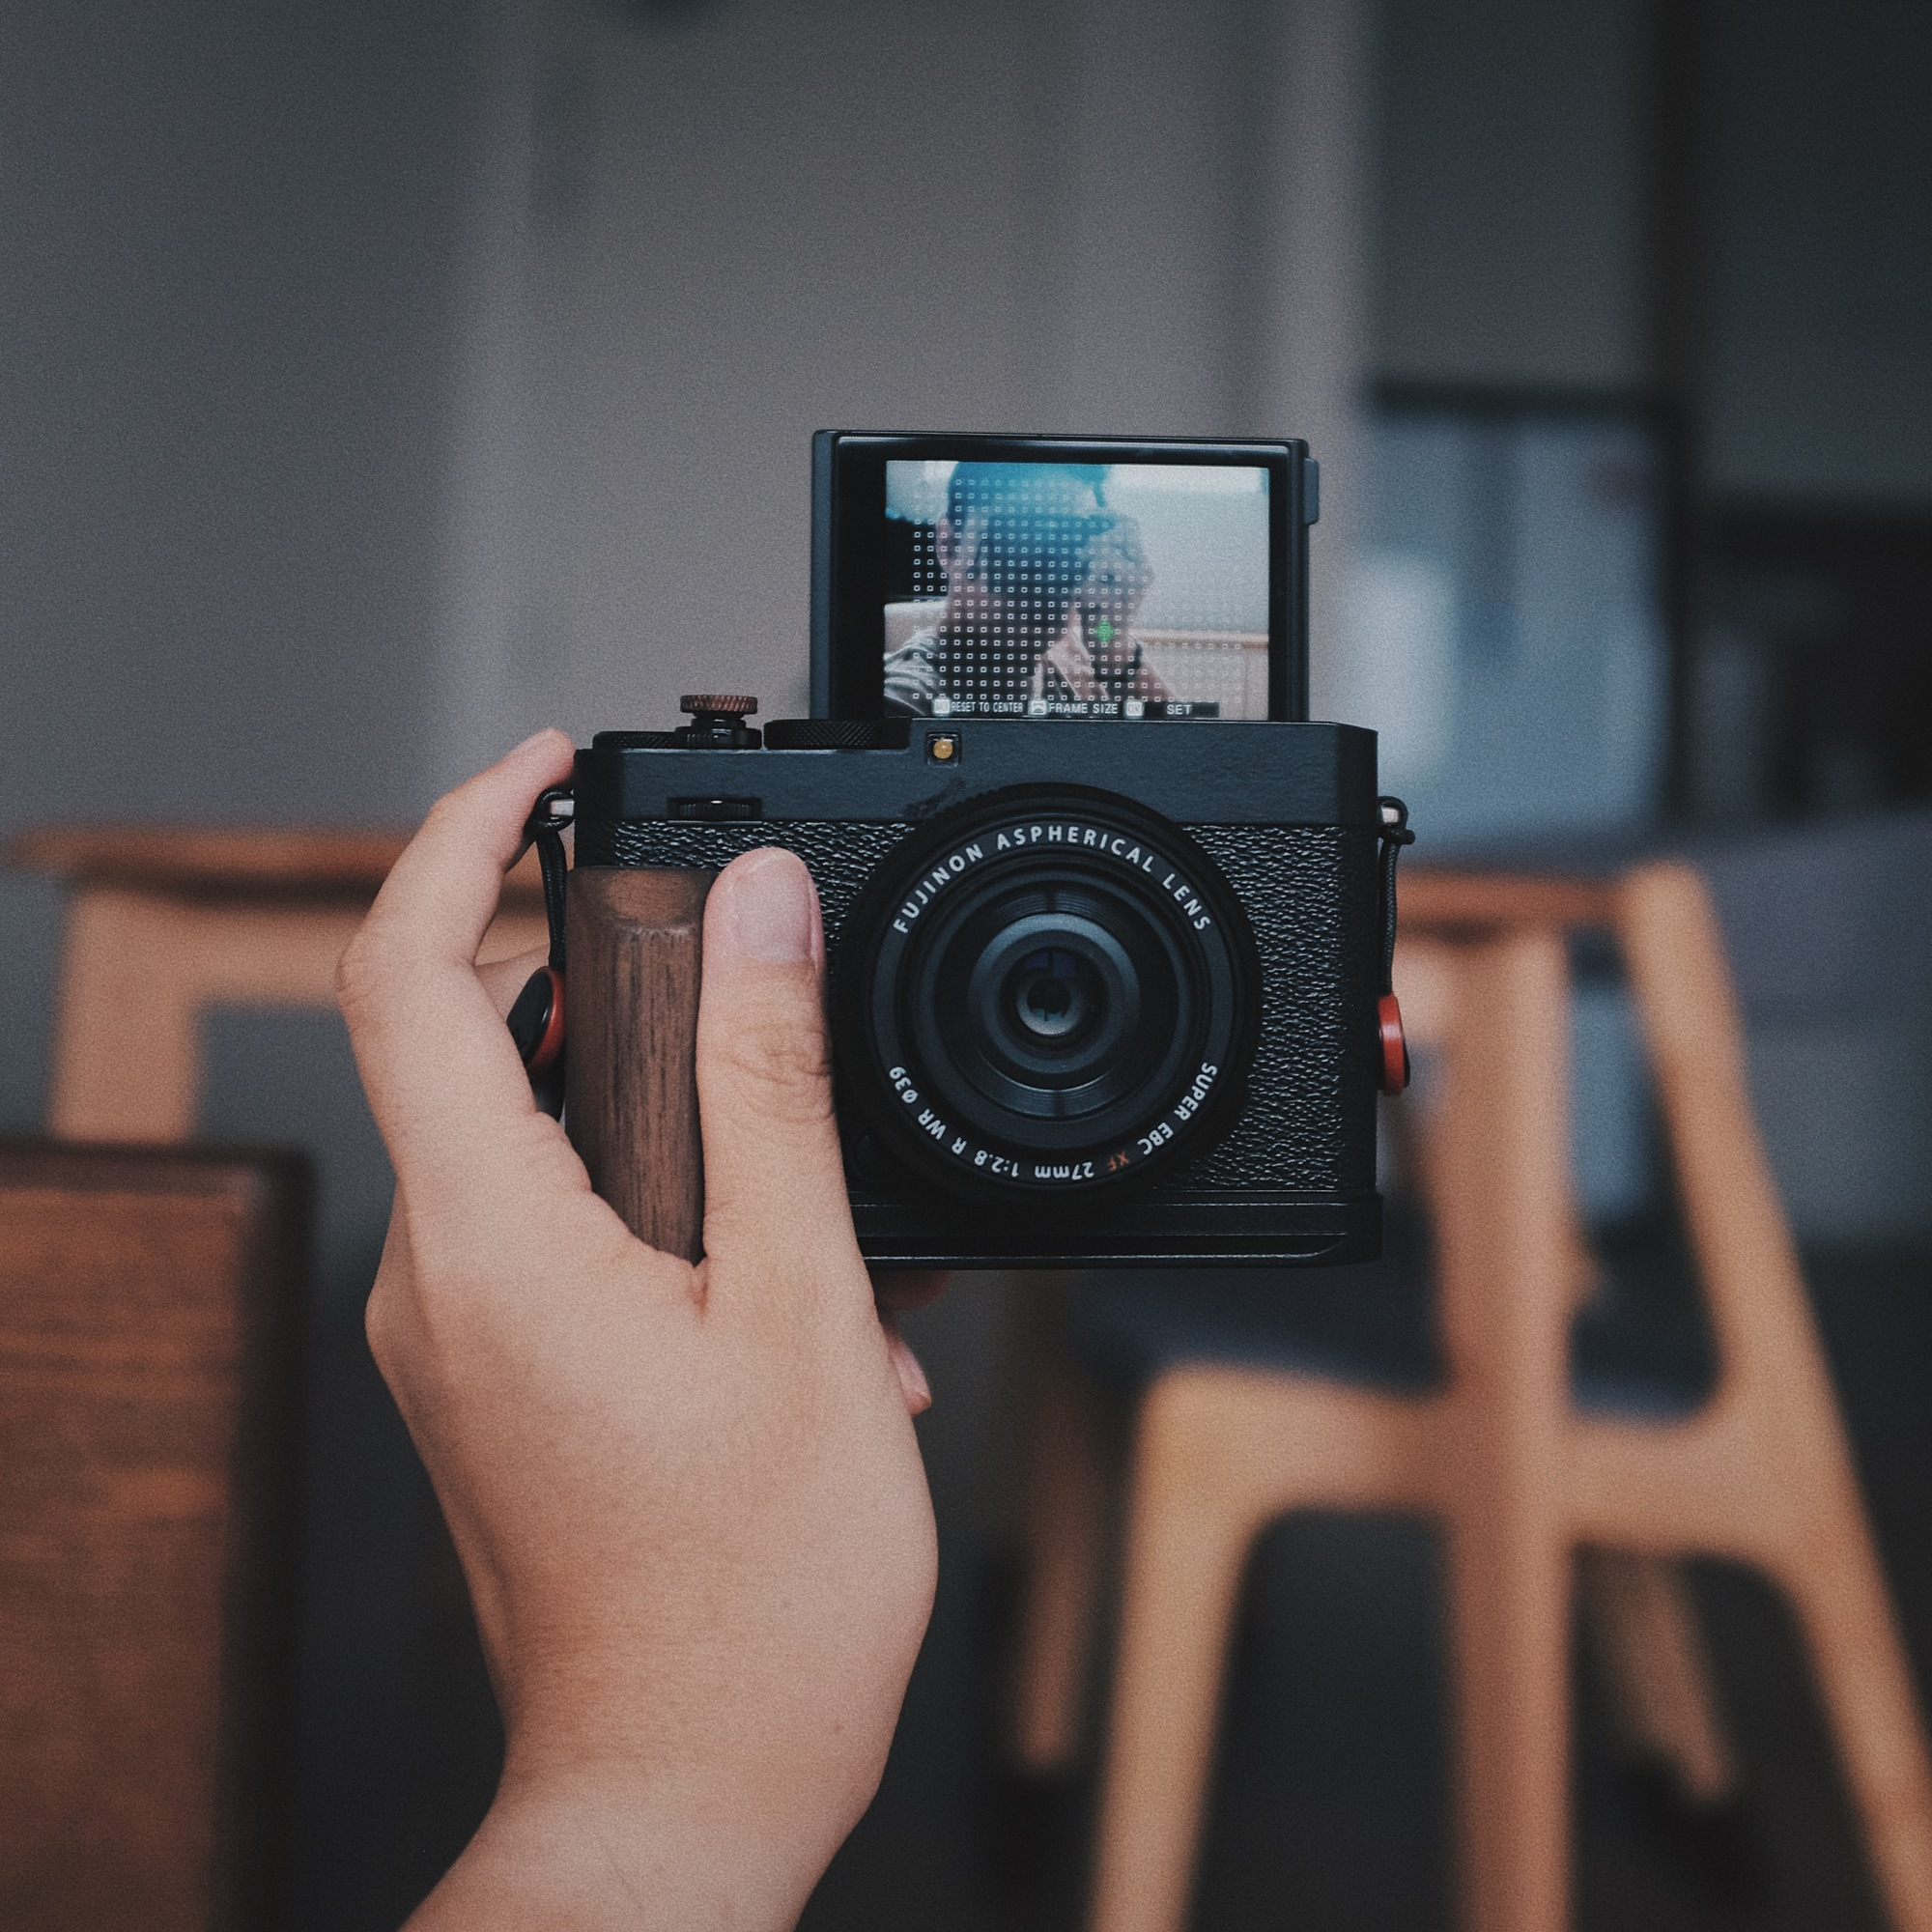
\includegraphics[width=\linewidth]{\envfinaldir/coverpic-prod.jpg}\par
            % \vskip 30pt
            \vfill

            \normalsize\rmfamily\scshape
            \copyright{} The Web Digest Project \hfill\large \envdatestr
        \end{center}
    \end{titlepage}
    % \restoregeometry
}
\newcommand{\simplehref}[1]{%
    \textcolor{blue!80!green}{\href{#1}{#1}}%
}
\renewcommand{\contentsname}{\center\Huge\sffamily\bfseries Contents\par\vskip 20pt}
\newcounter{ipartcounter}
\setcounter{ipartcounter}{0}
\newcommand{\ipart}[1]{
    % \vskip 20pt
    \clearpage
    \stepcounter{ipartcounter}
    \phantomsection
    \addcontentsline{toc}{chapter}{#1}
    % \begin{center}
    %     \Huge
    %     \sffamily\bfseries
    %     #1
    % \end{center}
    % \vskip 20pt plus 7pt
}
\newcounter{ichaptercounter}
\setcounter{ichaptercounter}{0}
\newcommand{\ichapter}[1]{
    % \vskip 20pt
    \clearpage
    \stepcounter{ichaptercounter}
    \phantomsection
    \addcontentsline{toc}{section}{\numberline{\arabic{ichaptercounter}}#1}
    \begin{center}
        \Huge
        \sffamily\bfseries
        #1
    \end{center}
    \vskip 20pt plus 7pt
}
\newcommand{\entrytitlefont}[1]{\subsection*{\raggedright\Large\sffamily\bfseries#1}}
\newcommand{\entryitemGeneric}[2]{
    % argv: title, url
    \parbox{\linewidth}{
        \entrytitlefont{#1}\par\vskip 5pt
        \footnotesize\ttfamily\mdseries
        \simplehref{#2}
    }\vskip 11pt plus 11pt minus 1pt
}
\newcommand{\entryitemGithub}[3]{
    % argv: title, url, desc
    \parbox{\linewidth}{
        \entrytitlefont{#1}\par\vskip 5pt
        \footnotesize\ttfamily\mdseries
        \simplehref{#2}\par\vskip 5pt
        \small\rmfamily\mdseries#3
    }\vskip 11pt plus 11pt minus 1pt
}
\newcommand{\entryitemAp}[3]{
    % argv: title, url, desc
    \parbox{\linewidth}{
        \entrytitlefont{#1}\par\vskip 5pt
        \footnotesize\ttfamily\mdseries
        \simplehref{#2}\par\vskip 5pt
        \small\rmfamily\mdseries#3
    }\vskip 11pt plus 11pt minus 1pt
}
\newcommand{\entryitemHackernews}[3]{
    % argv: title, hnurl, rawurl
    % \parbox{\linewidth}{
    %     \entrytitlefont{#1}\par\vskip 5pt
    %     \footnotesize\ttfamily\mdseries
    %     \simplehref{#3}\par
    %     \textcolor{black!50}{\href{#2}{#2}}
    % }\vskip 11pt plus 11pt minus 1pt
    \begin{minipage}{\linewidth}
            \entrytitlefont{#1}\par\vskip 5pt
            \footnotesize\ttfamily\mdseries
            \simplehref{#3}\par
            \textcolor{black!50}{\href{#2}{#2}}
    \end{minipage}\par\vskip 11pt plus 11pt minus 1pt
}







\begin{document}

\makeheader

\tableofcontents\clearpage




\ipart{Developers}
\ichapter{Hacker News}
\entryitemTwoLinks{Nice Things with SVG}{https://news.ycombinator.com/item?id=43666439}{https://fuma-nama.vercel.app/blog/svg-art}

\entryitemTwoLinks{Air pollution fell substantially as Paris restricted car traffic}{https://news.ycombinator.com/item?id=43665793}{https://www.washingtonpost.com/climate-solutions/2025/04/12/air-pollution-paris-health-cars/}

\entryitemTwoLinks{Tunarr: Create and configure live TV channels from media on your servers}{https://news.ycombinator.com/item?id=43665201}{https://tunarr.com/}

\entryitemTwoLinks{Emacs Lisp Elements}{https://news.ycombinator.com/item?id=43665046}{https://protesilaos.com/emacs/emacs-lisp-elements}

\entryitemTwoLinks{Apple, Nvidia, Dell, and Others Get a Tariffs Exemption Under New Rules}{https://news.ycombinator.com/item?id=43664665}{https://www.barrons.com/articles/tariffs-exclusions-exemptions-apple-nvidia-dell-smartphones-pcs-b2e069ff}

\entryitemTwoLinks{"Slow Pay, Low Pay or No Pay": Blue Cross Approved Surgeries Then Refused to Pay}{https://news.ycombinator.com/item?id=43664660}{https://www.propublica.org/article/blue-cross-blue-shield-louisiana-insurance-lawsuit-breast-cancer-doctors}

\entryitemTwoLinks{Trump exempts phones, computers, chips from 'reciprocal' tariffs}{https://news.ycombinator.com/item?id=43664121}{https://www.bloomberg.com/news/articles/2025-04-12/trump-exempts-phones-computers-chips-from-reciprocal-tariffs}

\entryitemTwoLinks{Charts.css}{https://news.ycombinator.com/item?id=43663880}{https://chartscss.org/}

\entryitemTwoLinks{Open source and self hostable/private file converter}{https://news.ycombinator.com/item?id=43663865}{https://vert.sh}

\entryitemTwoLinks{AI can't stop making up software dependencies and sabotaging everything}{https://news.ycombinator.com/item?id=43663777}{https://www.theregister.com/2025/04/12/ai\_code\_suggestions\_sabotage\_supply\_chain/}

\entryitemTwoLinks{\$70M in 60 Seconds: How Insider Info Helped Someone 28x Their Money}{https://news.ycombinator.com/item?id=43661680}{https://data-and-politics.ghost.io/70-million-in-60-seconds-how-insider-information-helped-someone-28x-their-money/}

\entryitemTwoLinks{Rust to C compiler – 95.9\% test pass rate, odd platforms}{https://news.ycombinator.com/item?id=43661329}{https://fractalfir.github.io/generated\_html/cg\_clr\_odd\_platforms.html}

\entryitemTwoLinks{Google is winning on every AI front}{https://news.ycombinator.com/item?id=43661235}{https://www.thealgorithmicbridge.com/p/google-is-winning-on-every-ai-front}

\entryitemTwoLinks{That groan you hear is users' reaction to Recall going back into Windows}{https://news.ycombinator.com/item?id=43660914}{https://arstechnica.com/security/2025/04/microsoft-is-putting-privacy-endangering-recall-back-into-windows-11/}

\entryitemTwoLinks{You might not need WebSockets}{https://news.ycombinator.com/item?id=43659370}{https://hntrl.io/posts/you-dont-need-websockets/}

\entryitemTwoLinks{Vacheron Constantin breaks the world record for most complicated wristwatch}{https://news.ycombinator.com/item?id=43659365}{https://www.hodinkee.com/articles/introducing-vacheron-constantin-les-cabinotiers-solaria}

\entryitemTwoLinks{AI Coding and the Peanut Butter and Jelly Problem}{https://news.ycombinator.com/item?id=43658794}{https://iamcharliegraham.substack.com/p/ai-coding-and-the-peanut-butter-and}

\entryitemTwoLinks{Googler... ex-Googler}{https://news.ycombinator.com/item?id=43658089}{https://nerdy.dev/ex-googler}

\entryitemTwoLinks{Germany creates 'super–high-tech ministry' for research, technology, aerospace}{https://news.ycombinator.com/item?id=43658060}{https://www.science.org/content/article/germany-creates-super-high-tech-ministry-research-technology-and-aerospace}

\entryitemTwoLinks{Social Security Administration Moving Public Communications to X}{https://news.ycombinator.com/item?id=43657079}{https://www.wired.com/story/social-security-administration-regional-office-elon-musk-x/}\ichapter{Phoronix}
\entryitemGeneric{\hskip 0pt{}Linux 6.16 Could See AMD SEV-SNP SVSM vTPM Driver Merged For EPYC CPUs}{https://www.phoronix.com/news/Linux-SNP-SVSM-vTPM-Driver-Tip}

\entryitemGeneric{\hskip 0pt{}A Fresh Take On Virtual Swap Space Being Pursued For The Linux Kernel}{https://www.phoronix.com/news/Linux-Virtual-Swap-Space}

\entryitemGeneric{\hskip 0pt{}KDE Plasma 6.4 Lands Initial Support For The Wayland Session Restore Protocol}{https://www.phoronix.com/news/KDE-Wayland-Session-Restore}

\entryitemGeneric{\hskip 0pt{}LibreOffice 25.8 Landing Many Patches For Improving Qt Toolkit Integration}{https://www.phoronix.com/news/LibreOffice-25.8-Qt-Weld}

\entryitemGeneric{\hskip 0pt{}NVIDIA Upstreaming Work For Linux On Their Smart Switch SN4280, SN5610, SN5640}{https://www.phoronix.com/news/Smart-Switch-SN4280-Linux}

\entryitemGeneric{\hskip 0pt{}GNOME Now Has A Second Core App Written In TypeScript}{https://www.phoronix.com/news/GNOME-2nd-Core-App-TypeScript}

\entryitemGeneric{\hskip 0pt{}AMD Releases ROCm 6.4 Without Any Official RDNA4 Support}{https://www.phoronix.com/news/AMD-ROCm-6.4-Released}

\entryitemGeneric{\hskip 0pt{}Running Linux 6.15 vs. 6.14 Performance With The AMD Ryzen AI 7 PRO 360}{https://www.phoronix.com/news/Linux-6.15-Ryzen-AI-7-PRO-360}

\entryitemGeneric{\hskip 0pt{}Intel Preps VRR Refactoring For Linux 6.16, More Xe3 Panther Lake Display Enablement}{https://www.phoronix.com/news/Intel-DRM-Next-Linux-6.16-1}\ichapter{Dribbble}
\entryitemGeneric{\hskip 0pt{}Chat App - Two Pages of Sketches}{https://dribbble.com/shots/25890352-Chat-App-Two-Pages-of-Sketches}

\entryitemGeneric{\hskip 0pt{}Nite Riot®\_Film Production // Case Study\_Vol.2.0}{https://dribbble.com/shots/25889874-Nite-Riot-Film-Production-Case-Study-Vol-2-0}

\entryitemGeneric{\hskip 0pt{}Lion}{https://dribbble.com/shots/25884438-Lion}

\entryitemGeneric{\hskip 0pt{}Adobe Acrobat Logo Redesign Concept}{https://dribbble.com/shots/25884888-Adobe-Acrobat-Logo-Redesign-Concept}

\entryitemGeneric{\hskip 0pt{}Fintech Web Design \& Landing Page for Puzzle}{https://dribbble.com/shots/25652139-Fintech-Web-Design-Landing-Page-for-Puzzle}

\entryitemGeneric{\hskip 0pt{}Web Design Crypto Trading}{https://dribbble.com/shots/25879747-Web-Design-Crypto-Trading}

\entryitemGeneric{\hskip 0pt{}Monster Pony Wooden toy}{https://dribbble.com/shots/25880300-Monster-Pony-Wooden-toy}

\entryitemGeneric{\hskip 0pt{}Educate AI Logo Design - Letter E, Monogram, Education}{https://dribbble.com/shots/25879659-Educate-AI-Logo-Design-Letter-E-Monogram-Education}

\entryitemGeneric{\hskip 0pt{}Hawkridge}{https://dribbble.com/shots/25877367-Hawkridge}

\entryitemGeneric{\hskip 0pt{}UI Design for Cargo Delivery Company}{https://dribbble.com/shots/25874804-UI-Design-for-Cargo-Delivery-Company}

\entryitemGeneric{\hskip 0pt{}Nite Riot®\_Film Production // Case Study\_Vol.1.0}{https://dribbble.com/shots/25874978-Nite-Riot-Film-Production-Case-Study-Vol-1-0}

\entryitemGeneric{\hskip 0pt{}UltraSlot}{https://dribbble.com/shots/25875506-UltraSlot}

\entryitemGeneric{\hskip 0pt{}Sidekick Ai 3d mascot}{https://dribbble.com/shots/25874949-Sidekick-Ai-3d-mascot}

\entryitemGeneric{\hskip 0pt{}🔐 Cybersecurity App Landing}{https://dribbble.com/shots/25873133--Cybersecurity-App-Landing}

\entryitemGeneric{\hskip 0pt{}Equati}{https://dribbble.com/shots/25858079-Equati}

\entryitemGeneric{\hskip 0pt{}Howzit}{https://dribbble.com/shots/25871668-Howzit}

\entryitemGeneric{\hskip 0pt{}Brainstorm}{https://dribbble.com/shots/25871145-Brainstorm}

\entryitemGeneric{\hskip 0pt{}Boxplates}{https://dribbble.com/shots/25869902-Boxplates}

\entryitemGeneric{\hskip 0pt{}Medieval H}{https://dribbble.com/shots/25862061-Medieval-H}

\entryitemGeneric{\hskip 0pt{}Nord Print Logo Design - Northern Star, Paper, Print, Printing}{https://dribbble.com/shots/25867726-Nord-Print-Logo-Design-Northern-Star-Paper-Print-Printing}

\entryitemGeneric{\hskip 0pt{}Spark illustrations}{https://dribbble.com/shots/25872229-Spark-illustrations}

\entryitemGeneric{\hskip 0pt{}Peach Media Logo Design}{https://dribbble.com/shots/25869696-Peach-Media-Logo-Design}

\entryitemGeneric{\hskip 0pt{}Quill Pen mark}{https://dribbble.com/shots/25871430-Quill-Pen-mark}

\entryitemGeneric{\hskip 0pt{}Skype Logo Redesign Concept}{https://dribbble.com/shots/25869984-Skype-Logo-Redesign-Concept}


\ipart{Developers~~~~(zh-Hans)}
\ichapter{Solidot}
\entryitemGeneric{\hskip 0pt{}生活在 4.36 亿年前的古鱼以袁隆平名字命名}{https://www.solidot.org/story?sid=81029}

\entryitemGeneric{\hskip 0pt{}AI 购物应用 CEO 被控欺诈,AI 的背后其实是人}{https://www.solidot.org/story?sid=81028}

\entryitemGeneric{\hskip 0pt{}微软真的准备推出 Recall}{https://www.solidot.org/story?sid=81027}

\entryitemGeneric{\hskip 0pt{}全球塑料回收率仅为 9\%}{https://www.solidot.org/story?sid=81026}

\entryitemGeneric{\hskip 0pt{}台湾澎湖发现的人骨化石被确认来自丹尼索瓦人}{https://www.solidot.org/story?sid=81025}

\entryitemGeneric{\hskip 0pt{}水道残留的抗焦虑药物改变野生鲑鱼的迁徙行为}{https://www.solidot.org/story?sid=81024}

\entryitemGeneric{\hskip 0pt{}英特尔 CPU 可能受中国对美关税政策影响}{https://www.solidot.org/story?sid=81023}

\entryitemGeneric{\hskip 0pt{}任天堂将越南制造的 Switch 2 游戏机几乎全部出口到美国}{https://www.solidot.org/story?sid=81022}

\entryitemGeneric{\hskip 0pt{}2024 年 58\% 的 PC 游戏收入来自微交易}{https://www.solidot.org/story?sid=81021}

\entryitemGeneric{\hskip 0pt{}科学家测量出中微子至今最精确质量上限 0.45 eV }{https://www.solidot.org/story?sid=81020}

\entryitemGeneric{\hskip 0pt{}美国政治措辞日益倾向于个人信念而不是事实}{https://www.solidot.org/story?sid=81019}

\entryitemGeneric{\hskip 0pt{}小鼠研究发现淀粉基微塑料可能存在健康风险}{https://www.solidot.org/story?sid=81018}

\entryitemGeneric{\hskip 0pt{}美国不想要孩子的人数在增长}{https://www.solidot.org/story?sid=81017}

\entryitemGeneric{\hskip 0pt{}Switch 2 推迟在华发售}{https://www.solidot.org/story?sid=81016}

\entryitemGeneric{\hskip 0pt{}美国暂停对等关税 90 天,对华关税提高到 125\%}{https://www.solidot.org/story?sid=81015}

\entryitemGeneric{\hskip 0pt{}科学家公布迄今最详尽的哺乳动物大脑连接图谱}{https://www.solidot.org/story?sid=81014}

\entryitemGeneric{\hskip 0pt{}Google 宣布了第七代 TPU 处理器 Ironwood}{https://www.solidot.org/story?sid=81013}

\entryitemGeneric{\hskip 0pt{}加固 Firefox 前端}{https://www.solidot.org/story?sid=81012}

\entryitemGeneric{\hskip 0pt{}OpenSSH 10.0 释出}{https://www.solidot.org/story?sid=81011}

\entryitemGeneric{\hskip 0pt{}中国将美国商品关税提高到 84\%}{https://www.solidot.org/story?sid=81010}\ichapter{V2EX}
\entryitemGeneric{\hskip 0pt{}[职场话题] 我感觉我已经无法离开 GPT 了}{https://www.v2ex.com/t/1125036}

\entryitemGeneric{\hskip 0pt{}[问与答] macOS safari 快手 web 端的问题}{https://www.v2ex.com/t/1125035}

\entryitemGeneric{\hskip 0pt{}[Windows] 一台式电脑想装多系统。}{https://www.v2ex.com/t/1125034}

\entryitemGeneric{\hskip 0pt{}[问与答] Macmini m4 扩容做家庭服务器,怎么比较合适?}{https://www.v2ex.com/t/1125033}

\entryitemGeneric{\hskip 0pt{}[分享创造] 我的第一款 App,用于制作拼贴画}{https://www.v2ex.com/t/1125032}

\entryitemGeneric{\hskip 0pt{}[问与答] 有什么简易开源的库存管理软件}{https://www.v2ex.com/t/1125031}

\entryitemGeneric{\hskip 0pt{}[Apple] 记一次体验很好的 trade in,并夸一波苹果的售后}{https://www.v2ex.com/t/1125030}

\entryitemGeneric{\hskip 0pt{}[问与答] iPhone 如何限制某个 App 只能走数据网络?不能走 WiFi?}{https://www.v2ex.com/t/1125029}

\entryitemGeneric{\hskip 0pt{}[macOS] b 站的视频为什么暂停后可以直接复制视频中的文字,这是 b 站的功能还是 MacOS 提供的接口?}{https://www.v2ex.com/t/1125028}

\entryitemGeneric{\hskip 0pt{}[问与答] 有没有摩友,想买个二手 adv, v 友有什么性价比推荐吗?}{https://www.v2ex.com/t/1125027}

\entryitemGeneric{\hskip 0pt{}[问与答] pixel4a 5G 的屏幕摔了一下绿屏了 哪里可以找到靠谱的呀}{https://www.v2ex.com/t/1125026}

\entryitemGeneric{\hskip 0pt{}[程序员] cloudflare 对象存储,使用自定义域名之后速度降得厉害}{https://www.v2ex.com/t/1125025}

\entryitemGeneric{\hskip 0pt{}[分享发现] 小阿里云 claw 推出免费容器云,可以直接免费部署 alist 等等}{https://www.v2ex.com/t/1125023}

\entryitemGeneric{\hskip 0pt{}[奇思妙想] mcp 是不是可以实现订阅付费知识库啊,感觉搜索还是不太灵,可能会有 知识星球 之类的付费内容圈子的 mcp 吗}{https://www.v2ex.com/t/1125021}

\entryitemGeneric{\hskip 0pt{}[Cloudflare] cloudflare 对象存储,使用自定义域名之后限速得厉害}{https://www.v2ex.com/t/1125019}

\entryitemGeneric{\hskip 0pt{}[IPFS] 搜索 IPFS 上的内容}{https://www.v2ex.com/t/1125018}

\entryitemGeneric{\hskip 0pt{}[Windows] 请问大家如何看待网上各种大神制作的 Windows 精简版?}{https://www.v2ex.com/t/1125017}

\entryitemGeneric{\hskip 0pt{}[问与答] 新屋准备装水电了,求推荐网线和水晶头品牌}{https://www.v2ex.com/t/1125016}

\entryitemGeneric{\hskip 0pt{}[问与答] 通常移动硬盘使用什么文件系统格式?}{https://www.v2ex.com/t/1125015}

\entryitemGeneric{\hskip 0pt{}[问与答] 自媒体短视频创作领域已经形成了非常大的经济体量,有哪些比较好的朝着一站式素材供给的产品出现吗?}{https://www.v2ex.com/t/1125014}

\entryitemGeneric{\hskip 0pt{}[酷工作] [杭州] [知名机器人公司] 嵌入式软件 TL、软件 TL、中间件开发工程师、产品经理、硬件研发总监等多个职位招人,欢迎有兴趣的同学投递}{https://www.v2ex.com/t/1125013}

\entryitemGeneric{\hskip 0pt{}[程序员] 618 期间电脑配置推荐}{https://www.v2ex.com/t/1125012}

\entryitemGeneric{\hskip 0pt{}[问与答] 兄弟姐妹们,帮忙识别下这个啥字体}{https://www.v2ex.com/t/1125011}

\entryitemGeneric{\hskip 0pt{}[程序员] 我的家庭监控的安全使用办法}{https://www.v2ex.com/t/1125010}

\entryitemGeneric{\hskip 0pt{}[VPS] 关于 ClawCloud JP 日本的延迟测试}{https://www.v2ex.com/t/1125008}

\entryitemGeneric{\hskip 0pt{}[问与答] 想做一个只可以发纯文字信息的分类信息小程序,哪个程序好?}{https://www.v2ex.com/t/1125007}

\entryitemGeneric{\hskip 0pt{}[程序员] 肝了一篇 Google Agent2Agent 协议的介绍}{https://www.v2ex.com/t/1125006}

\entryitemGeneric{\hskip 0pt{}[问与答] 有 Linux 控制的智能插座吗}{https://www.v2ex.com/t/1125005}

\entryitemGeneric{\hskip 0pt{}[VPS] claw cloud 的免费容器}{https://www.v2ex.com/t/1125003}

\entryitemGeneric{\hskip 0pt{}[分享发现] ClawCloud 免费容器,不用买 vps 了,暂时不需要验卡!}{https://www.v2ex.com/t/1125002}

\entryitemGeneric{\hskip 0pt{}[推广] [推广]快递 100 寄快递全国五元起寄}{https://www.v2ex.com/t/1125001}

\entryitemGeneric{\hskip 0pt{}[优惠信息] 网易云音乐黑胶 VIP 免费送天数}{https://www.v2ex.com/t/1125000}

\entryitemGeneric{\hskip 0pt{}[分享创造] 完成一个基于 AI 的调色板在线网站 ColorMagic.club}{https://www.v2ex.com/t/1124999}

\entryitemGeneric{\hskip 0pt{}[分享创造] 盘小子:一站式网盘资源搜索神器来了(已开源)}{https://www.v2ex.com/t/1124998}

\entryitemGeneric{\hskip 0pt{}[宽带症候群] 现在连同省跨运营商都限制吗}{https://www.v2ex.com/t/1124997}

\entryitemGeneric{\hskip 0pt{}[问与答] 求推荐 b 站 tv 版 app}{https://www.v2ex.com/t/1124996}

\entryitemGeneric{\hskip 0pt{}[问与答] 彩云天气后来是不是换了开发商了?}{https://www.v2ex.com/t/1124995}

\entryitemGeneric{\hskip 0pt{}[全球工单系统] 大众点评的部分微服务挂了?}{https://www.v2ex.com/t/1124993}

\entryitemGeneric{\hskip 0pt{}[分享创造] TabTab docs 站点}{https://www.v2ex.com/t/1124991}

\entryitemGeneric{\hskip 0pt{}[分享创造] 分享一下自己的博客,最近大更新了一番}{https://www.v2ex.com/t/1124990}

\entryitemGeneric{\hskip 0pt{}[分享发现] 剃须刀到底应该怎么清洗}{https://www.v2ex.com/t/1124989}

\entryitemGeneric{\hskip 0pt{}[分享发现] 终于发现了一个符合我需求的摄影博客项目, exif-photo-blog}{https://www.v2ex.com/t/1124988}

\entryitemGeneric{\hskip 0pt{}[程序员] adk 怎么样,能否替代 langchain langgraph 等其他 agent 框架}{https://www.v2ex.com/t/1124987}

\entryitemGeneric{\hskip 0pt{}[问与答] 5G 唯一受益者的这个言论想要表达什么意思?}{https://www.v2ex.com/t/1124986}

\entryitemGeneric{\hskip 0pt{}[iPhone] 中國雷達回波圖 app}{https://www.v2ex.com/t/1124985}

\entryitemGeneric{\hskip 0pt{}[优惠信息] Chatwise 8 折 限时优惠}{https://www.v2ex.com/t/1124984}

\entryitemGeneric{\hskip 0pt{}[分享发现] 抖音商城,不同版本的抖音竟然直播间价格不同,疑似杀熟}{https://www.v2ex.com/t/1124982}

\entryitemGeneric{\hskip 0pt{}[分享发现] 在家窝着,让 AI 帮我修电视}{https://www.v2ex.com/t/1124981}

\entryitemGeneric{\hskip 0pt{}[远程工作] [远程办公全职] NLP 算法急招 年薪 60 万+,也有其他算法岗}{https://www.v2ex.com/t/1124980}

\entryitemGeneric{\hskip 0pt{}[VPS] 求推荐一个国外的 vps。}{https://www.v2ex.com/t/1124979}


\ipart{Generic News}







\clearpage
\leavevmode\vfill
\footnotesize

Copyright \copyright{} 2023-2025 Neruthes and other contributors.

This document is published with CC BY-NC-ND 4.0 license.

The entries listed in this newsletter may be copyrighted by their respective creators.

This newsletter is generated by the Web Digest project.

The newsletters are also delivered via Telegram channel \CJKunderline{\href{https://t.me/webdigestchannel}{https://t.me/webdigestchannel}}.\\
RSS feed is available at \CJKunderline{\href{https://webdigest.pages.dev/rss.xml}{https://webdigest.pages.dev/rss.xml}}.

This newsletter is available in PDF at
\CJKunderline{\href{https://webdigest.pages.dev/}{https://webdigest.pages.dev/}}.

The source code being used to generate this newsletter is available at\\
\CJKunderline{\href{https://github.com/neruthes/webdigest}{https://github.com/neruthes/webdigest}}.

This newsletter is also available in
\CJKunderline{\href{http://webdigest.pages.dev/readhtml/\envyear/WebDigest-20250413.html}{HTML}} and
\CJKunderline{\href{https://github.com/neruthes/webdigest/blob/master/markdown/\envyear/WebDigest-20250413.md}{Markdown}}.


\coverpic{https://unsplash.com/photos/man-wearing-a-fur-hat-and-coat-looks-directly-at-camera-x4ldh59QJ1s}{Fadhil Abhimantra}


\end{document}
